\documentclass{amsart}

\usepackage[french]{babel}
\usepackage{graphicx}
\usepackage{float}

\newtheorem{theorem}{Théorème}[section]
\newtheorem{lemma}[theorem]{Lemme}

\theoremstyle{definition}
\newtheorem{definition}[theorem]{Définition}
\newtheorem{example}[theorem]{Exemple}
\newtheorem{xca}[theorem]{Exercice}

\theoremstyle{remark}
\newtheorem{remark}[theorem]{Remarque}

\numberwithin{equation}{section}

%    Absolute value notation
\newcommand{\abs}[1]{\lvert#1\rvert}

%    Blank box placeholder for figures (to avoid requiring any
%    particular graphics capabilities for printing this document).
\newcommand{\blankbox}[2]{%
  \parbox{\columnwidth}{\centering
%    Set fboxsep to 0 so that the actual size of the box will match the
%    given measurements more closely.
    \setlength{\fboxsep}{0pt}%
    \fbox{\raisebox{0pt}[#2]{\hspace{#1}}}%
  }%
}

\renewcommand*{\overrightarrow}[1]{\vbox{\halign{##\cr 
  \tiny\rightarrowfill\cr\noalign{\nointerlineskip\vskip1pt} 
  $#1\mskip2mu$\cr}}}

\begin{document}

\title{Électron libre}

\author{Bellevue (BLV)}

\begin{abstract}
    Cet article contient la résolution de nombreuses questions du problème \og Électron libre \fg{} de la quatorzième édition du Tournoi Français
    des Jeunes Mathématiciennes et Mathématiciens. La résolution de problème est composé de lemmes, théorèmes et conjectures énoncés à la suite. 
    Notez que pour la résolution de certains problèmes dans un plan quelconque, on a jugé que la création d'un plan orthonormé ne présentait pas de soucis.

\end{abstract}

\maketitle

\tableofcontents

\section{Introduction}

Nicolas joue dispose d’un canon à électrons immergé dans un champ magnétique constant uniforme. À l'aide de son canon, il peut émettre un électron 
circulant alors à vitesse constante en décrivant un cercle dans le sens trigonométrique, que l'on a supposé de rayon 1. 

Il dispose aussi d’un bouton qui permet de faire faire demi-tour à l’électron tel qu'au moment où il appuie, la vitesse de l’électron reste la même 
mais progresse dans la direction opposée.

Le coeur du problème réside dans l'optimisation entre la longueur totale de la courbe de la trajectoire, du nombre d'appuies, ainsi que la restriction 
de la taille de la trajectoire selon l'espace.\newpage
\section{Définitions}

\begin{definition}
  On appelle \textbf{trajet} une courbe permettant de relier deux points $A,B$ dans un plan quelconque. Voici des exemples de trajets:

  \begin{figure}[H]
    \centering
    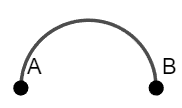
\includegraphics[scale=0.5]{circle.png}
    \caption{Un trajet circulaire.}
  \end{figure}

  \begin{figure}[H]
    \centering
    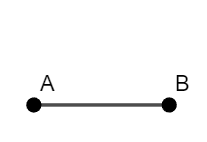
\includegraphics[scale=0.5]{line.png}
    \caption{Un trajet étant le segment [AB].}
  \end{figure}

  \begin{figure}[H]
    \centering
    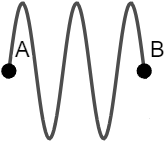
\includegraphics[scale=0.5]{sinus.png}
    \caption{Un trajet sinusoïdal.}
  \end{figure}
\end{definition}

\begin{definition}
  On appelle $\lambda(A,B)$ la longueur d'une courbe (trajet) dans un plan quelconque reliant deux points $A,B$. Dans le cadre de la courbe d'une fonction $f:\mathbb{R}\longrightarrow \mathbb{R}, x\longmapsto f(x)$,
  on considère donc que: \[\lambda(A,B)=\int_{x_a}^{x_b} \sqrt{1+{f^\prime}^2} \,dx\]
  
  (La démonstration est effectuée à la suite de l'article).
\end{definition}

\begin{definition}
  On appelle $n_{bouton}$ le nombre de fois que l'on appuie sur le bouton permettant de changer le sens trigonométrique de la trajectoire.
\end{definition}

\begin{definition}
  On appelle un \textbf{demi-cercle trigonométrique perpétuel} un trajet composée de plusieurs addition d'$1/2$ circonférence d'un cercle trigonométrique (soit $\pi$). Voici une illustration ci-dessous:
  
  \begin{figure}[H]
    \centering
    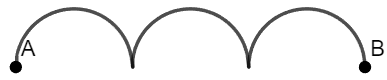
\includegraphics[scale=0.5]{demicircle.png}
    \caption{Un demi-cercle trigonométrique perpétuel répété 3 fois.}
  \end{figure}
\end{definition}

\begin{definition}
  On appelle \textbf{distance absolue} la plus petite distance séparant deux points $A,B$ dans un plan quelconque, soit le segment [AB] (Voir le \textbf{Théorème 3.3}.). On la note $d_{abs}$ avec $d_{abs}\in\mathbb{R^+}$ (une longueur étant toujours positive).
\end{definition}

\begin{definition}
  On appelle \textbf{distance minimale} la plus petite distance séparant deux points $A,B$ dans un plan quelconque, avec un trajet circulaire (ou de demi-cercles trigonométrique perpétuels). On la note $d_{min}$ avec $d_{min}\in\mathbb{R^+}$ (une longueur étant toujours positive).
\end{definition}

\section{Théorèmes utilitaires}

\begin{theorem}
  Soit $a,b\in\mathbb{R}$ avec $b>a$. Soit $f,g$ deux fonctions continues sur $]a,b[$ avec $f:\mathbb{R}\longrightarrow \mathbb{R}, x\longmapsto f(x)$ et $g:\mathbb{R}\longrightarrow \mathbb{R}, x\longmapsto g(x)$. Si $f(x)\geq g(x) \forall x\in]a,b[\implies$

  \[\int_{a}^{b}f(x) \,dx \geq \int_{a}^{b}g(x) \,dx\]
\end{theorem}

\begin{proof}
  Puisque $f(x)\geq g(x) \forall x\in]a,b[ \implies f(x)-g(x)\geq 0\forall x\in]a,b[ $. Par le théorème fondamental de l’analyse, si $f(x)$ est continue sur $]a,b[$, alors son intégral $F(b)-F(a)$ sur $]a,b[$ est définie comme : 
  \[F(b)-F(a) = \int_{a}^{b} f(x) , dx\]

  De même, l'intégral de $g$, $G(b)-G(a)$, est définie comme: \[G(b)-G(a) = \int_{a}^{b} g(x) , dx\]
  
  On sait aussi que, comme $f(x)-g(x)\geq0$, cela implique que l'aire en dessous de cette différence est supérieure à zéro. Intégrons cette inégalité de $a$ à $b$: \[\implies \int_{a}^{b} f(x) - g(x), dx \geq 0 \Leftrightarrow F(x)-G(x) \Biggr|_{a}^{b}\geq0 \Leftrightarrow F(b)-G(b) -(F(a)-G(a)) \geq 0 \]

  Soit donc:

  \[F(b)-F(a) \geq G(b)-G(a) \Leftrightarrow \int_{a}^{b}f(x) \,dx \le \int_{a}^{b}g(x) \,dx\]
\end{proof}

\begin{theorem}
  Soit $f$ une fonction tel que $f:\mathbb{R}\longrightarrow \mathbb{R}, x\longmapsto f(x)$. Soit $a,b\in\mathbb{R}$. On considère la longueur de la courbe de $f$ allant de $a$ à $b$ étant égale à:
  
  \[\lambda(a,b)=\int_{a}^{b} \sqrt{1+{f^\prime}^2} \,dx\]
\end{theorem}

\begin{proof}
  
\end{proof}

\begin{theorem}
  Soit $A,B$ deux points dans un plan quelconque. On admet que le trajet le plus court afin d'aller de $A$ à $B$ est une ligne droite.
\end{theorem}

\begin{proof}
  Considérons deux points $A,B$ dans un plan quelconque. Soit le repère orthonormé $(A;I;J)$ tel que \overrightarrow{AJ} $\perp$ \overrightarrow{AB}. On considère donc les points $A(x_a=0,y_a=0)$ et $B(x_b,y_b=0)$.
  
  Soit $f_q, f_q:\mathbb{R}\longrightarrow \mathbb{R}, x\longmapsto f_q(x)$, une fonction continue sur $[x_a,x_b]$ modélisant le trajet de $A$ à $B$ (n'étant pas une droite, avec $f_q(x)=0$ à $x_a$ et $x_b$, pour compléter la courbe). Soit $f_k, f_q:\mathbb{R}\longrightarrow \mathbb{R}, x\longmapsto 0$ une fonction
  continue sur $[x_a,x_b]$, $f_k\in\mathbb{R}$, modélisant la droite entre $A$ et $B$.
  
  En effectuant un raisonnement par l'absurde, supposons que $\exists f_q,f_q(x_a)=f_q(x_b)=0$ mais non $f_q(x)=0, \forall x\in\mathbb{R}$, tel que $\lambda_q(A,B) < \lambda_k(A,B)$.

  $0$ étant une constante, on sait que ${f_k}^\prime(x)=0$:

  \[\implies \lambda_k(A,B)=\int_{x_a}^{x_b}1 \,dx \Leftrightarrow \lambda_k(A,B)= x_b-x_a \]

  Or $f_q(x)\ne 0,\forall x\in\mathbb{R} \implies f_q(x)$ doit avoir une valeur dépendant de $x$ (et non pas juste d'une constante $k$ ou $kx, k\in\mathbb{R}$, car dans un tel cas, $f_q(x_a)\ne f_q(x_b)$). 

  \[\implies \lambda_q(A,B)=\int_{x_a}^{x_b}\sqrt{1+f_q{^\prime}(x)^2} \,dx\]

  Nous savons donc que: 

  \[1 < \sqrt{1+f_q{^\prime}(x)^2}\] 
  
  $\forall x \in \mathbb{R}$ car $f_q{^\prime}(x)^2> 0, \forall x \in \mathbb{R}$, avec la fonction racine carré étant croissante sur $\mathbb{R}$:

  \[\implies \int_{x_a}^{x_b}1 \,dx < \int_{x_a}^{x_b}\sqrt{1+f_q{^\prime}(x)^2} \,dx\] 
  
  (D'après le \textbf{Théorème 3.1}).

  On en déduit que $\lambda_k(A,B) < \lambda_q(A,B)$, soit le trajet le plus court pour aller de $A$ à $B$ étant une ligne droite.
\end{proof}

\section{Théorèmes pour la Question 1}

\begin{theorem}
  Dans le cas où $d_{abs}\le 2$, avec $n_{bouton}=0$, $d_{min}= 2sin^{-1}(\frac{d_{abs}}{2})$
\end{theorem}

\begin{proof}
  Pouvant choisir l'orientation initiale du canon, on sait que l'on peut former des arcs de cercles permettant d'atteindre $B$ à partir de $A$.
  Voici deux approches:\\

  \textbf{Approche 1}: On considère le repère orthonormé $(O;I;J)$ tel que \overrightarrow{OI} $\perp$ \overrightarrow{OJ}. On considère de même le cercle trigonométrique $C$ centré au point O et le point $A(1;0)$ inscrit dans C. Soit le point
  $B$ inscrit dans $C$ (sur sa circonférence).
  Soit $\theta$ l'angle séparant $A$ et $B$ à travers le cercle C.
  
  Nous pouvons donc former le triangle $\widehat{BOA}$ isocèle en $O$ avec $BO=1$, $OA=1$ et $AB=d_{abs}$. Soit $D$, milieu segment $[AB]$ tel que $OD$ coupe $\theta$ en deux. Nous avons donc deux triangles rectangles égaux $\widehat{ODA}$ et $\widehat{ODB}$.

  D'après les propriétés trigonométrique d'un triangle rectangle, nous avons:

  \[sin(\frac{\theta}{2})=\frac{d_{abs}}{2} \Leftrightarrow \theta = 2sin^{-1}(\frac{d_{abs}}{2})\]

  Étant dans un cercle trigonométrique, nous savons que $d_{min}=\theta$ (car $r=1$, $r$ étant le rayon du cercle), soit: 
  \[d_{min}=2sin^{-1}(\frac{d_{abs}}{2})\] \\

  Voici une illustration géométrique de la preuve:

  \begin{figure}[H]
    \centering
    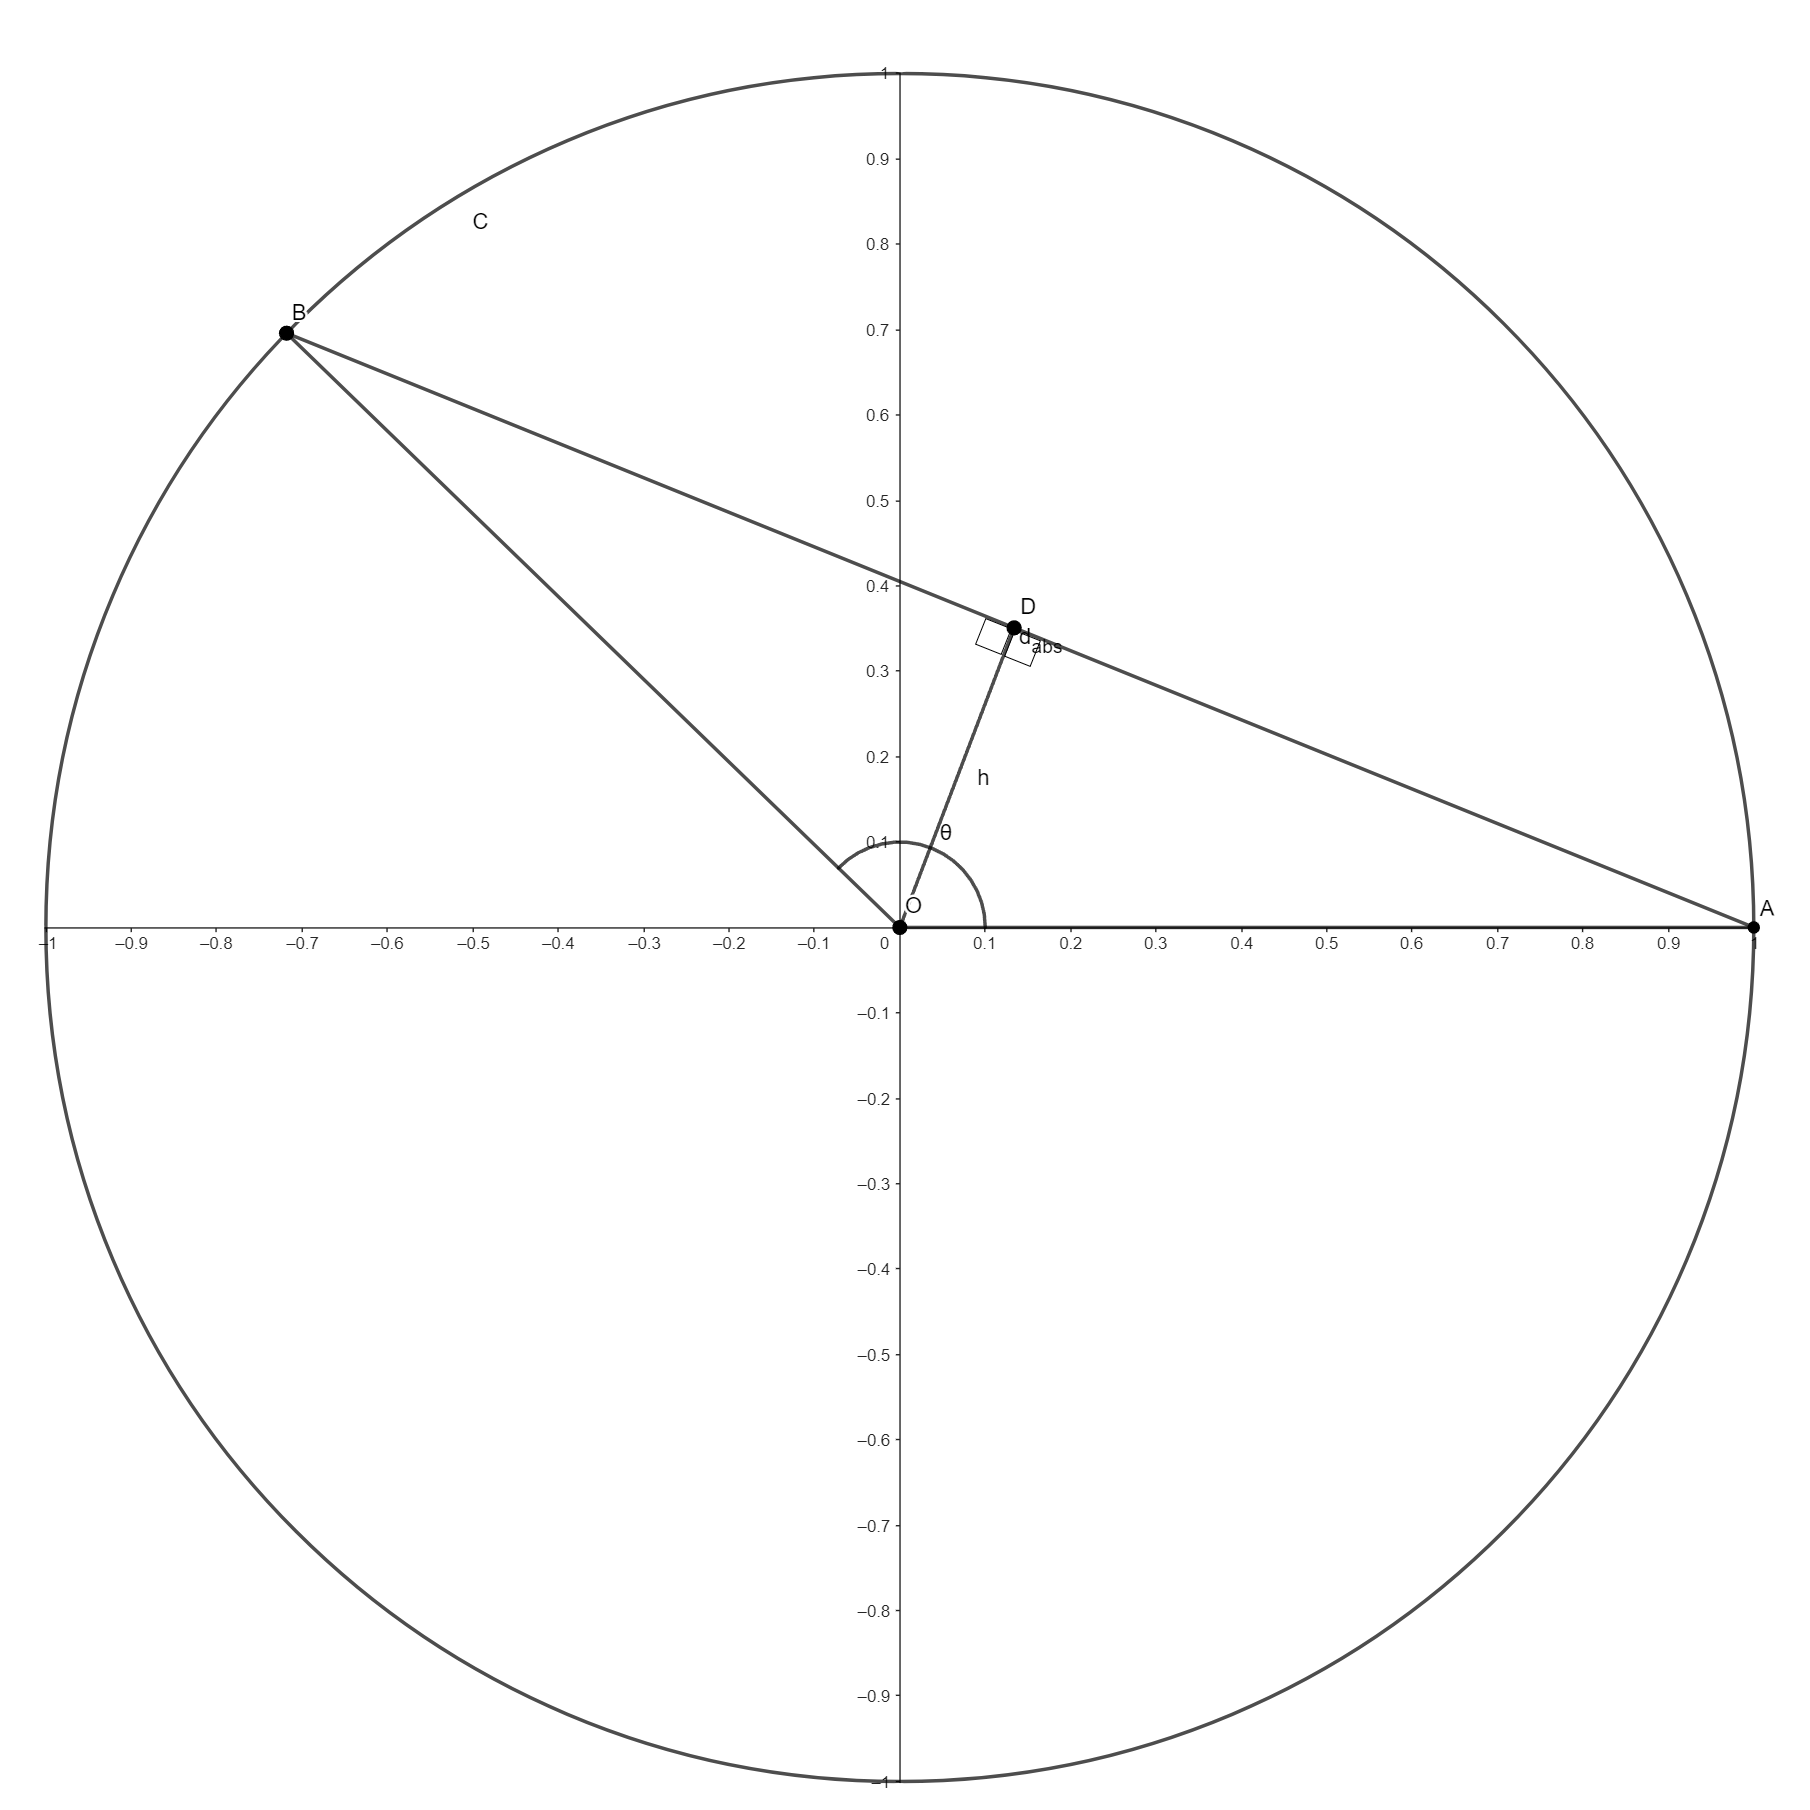
\includegraphics[scale=0.2]{angle.png}
    \caption{Un repère orthonormé avec le cercle trigonométrique $C$ de rayon $r=1$.}
  \end{figure}

  \textbf{Approche 2}: On considère de même le repère orthonormé $(O;I;J)$ tel que \overrightarrow{OI} $\perp$ \overrightarrow{OJ}. On considère de même le cercle trigonométrique $C$ centré au point O et le point $A(-1;0)$ inscrit dans C. Soit le point
  $B(x_b,y_b)$ inscrit dans $C$ (sur sa circonférence).

  Nous pouvons modéliser $C$ à partir de l'équation modélisant un cercle dans un repère orthonormé. Soit $r,x,y\in\mathbb{R}$ avec $y$ représentant les ordonnés, $x$ les abscisses et $r$ le rayon, tel que:
  \[r^2=y^2+x^2 \Leftrightarrow  y = \sqrt{r^2-x^2}\]

  À partir de cette égalité, nous considérons dans notre cas que $r=1$, car il s'agit du cercle trigonométrique. Nous pouvons définir la fonction $f,f:\mathbb{R}\longrightarrow \mathbb{R}, x\longmapsto \sqrt{1-x^2}, \forall x\in[-1;1]$.

  Voici une illustration géométrique de la courbe de $f$ ainsi que les points associés:

  \begin{figure}[H]
    \centering
    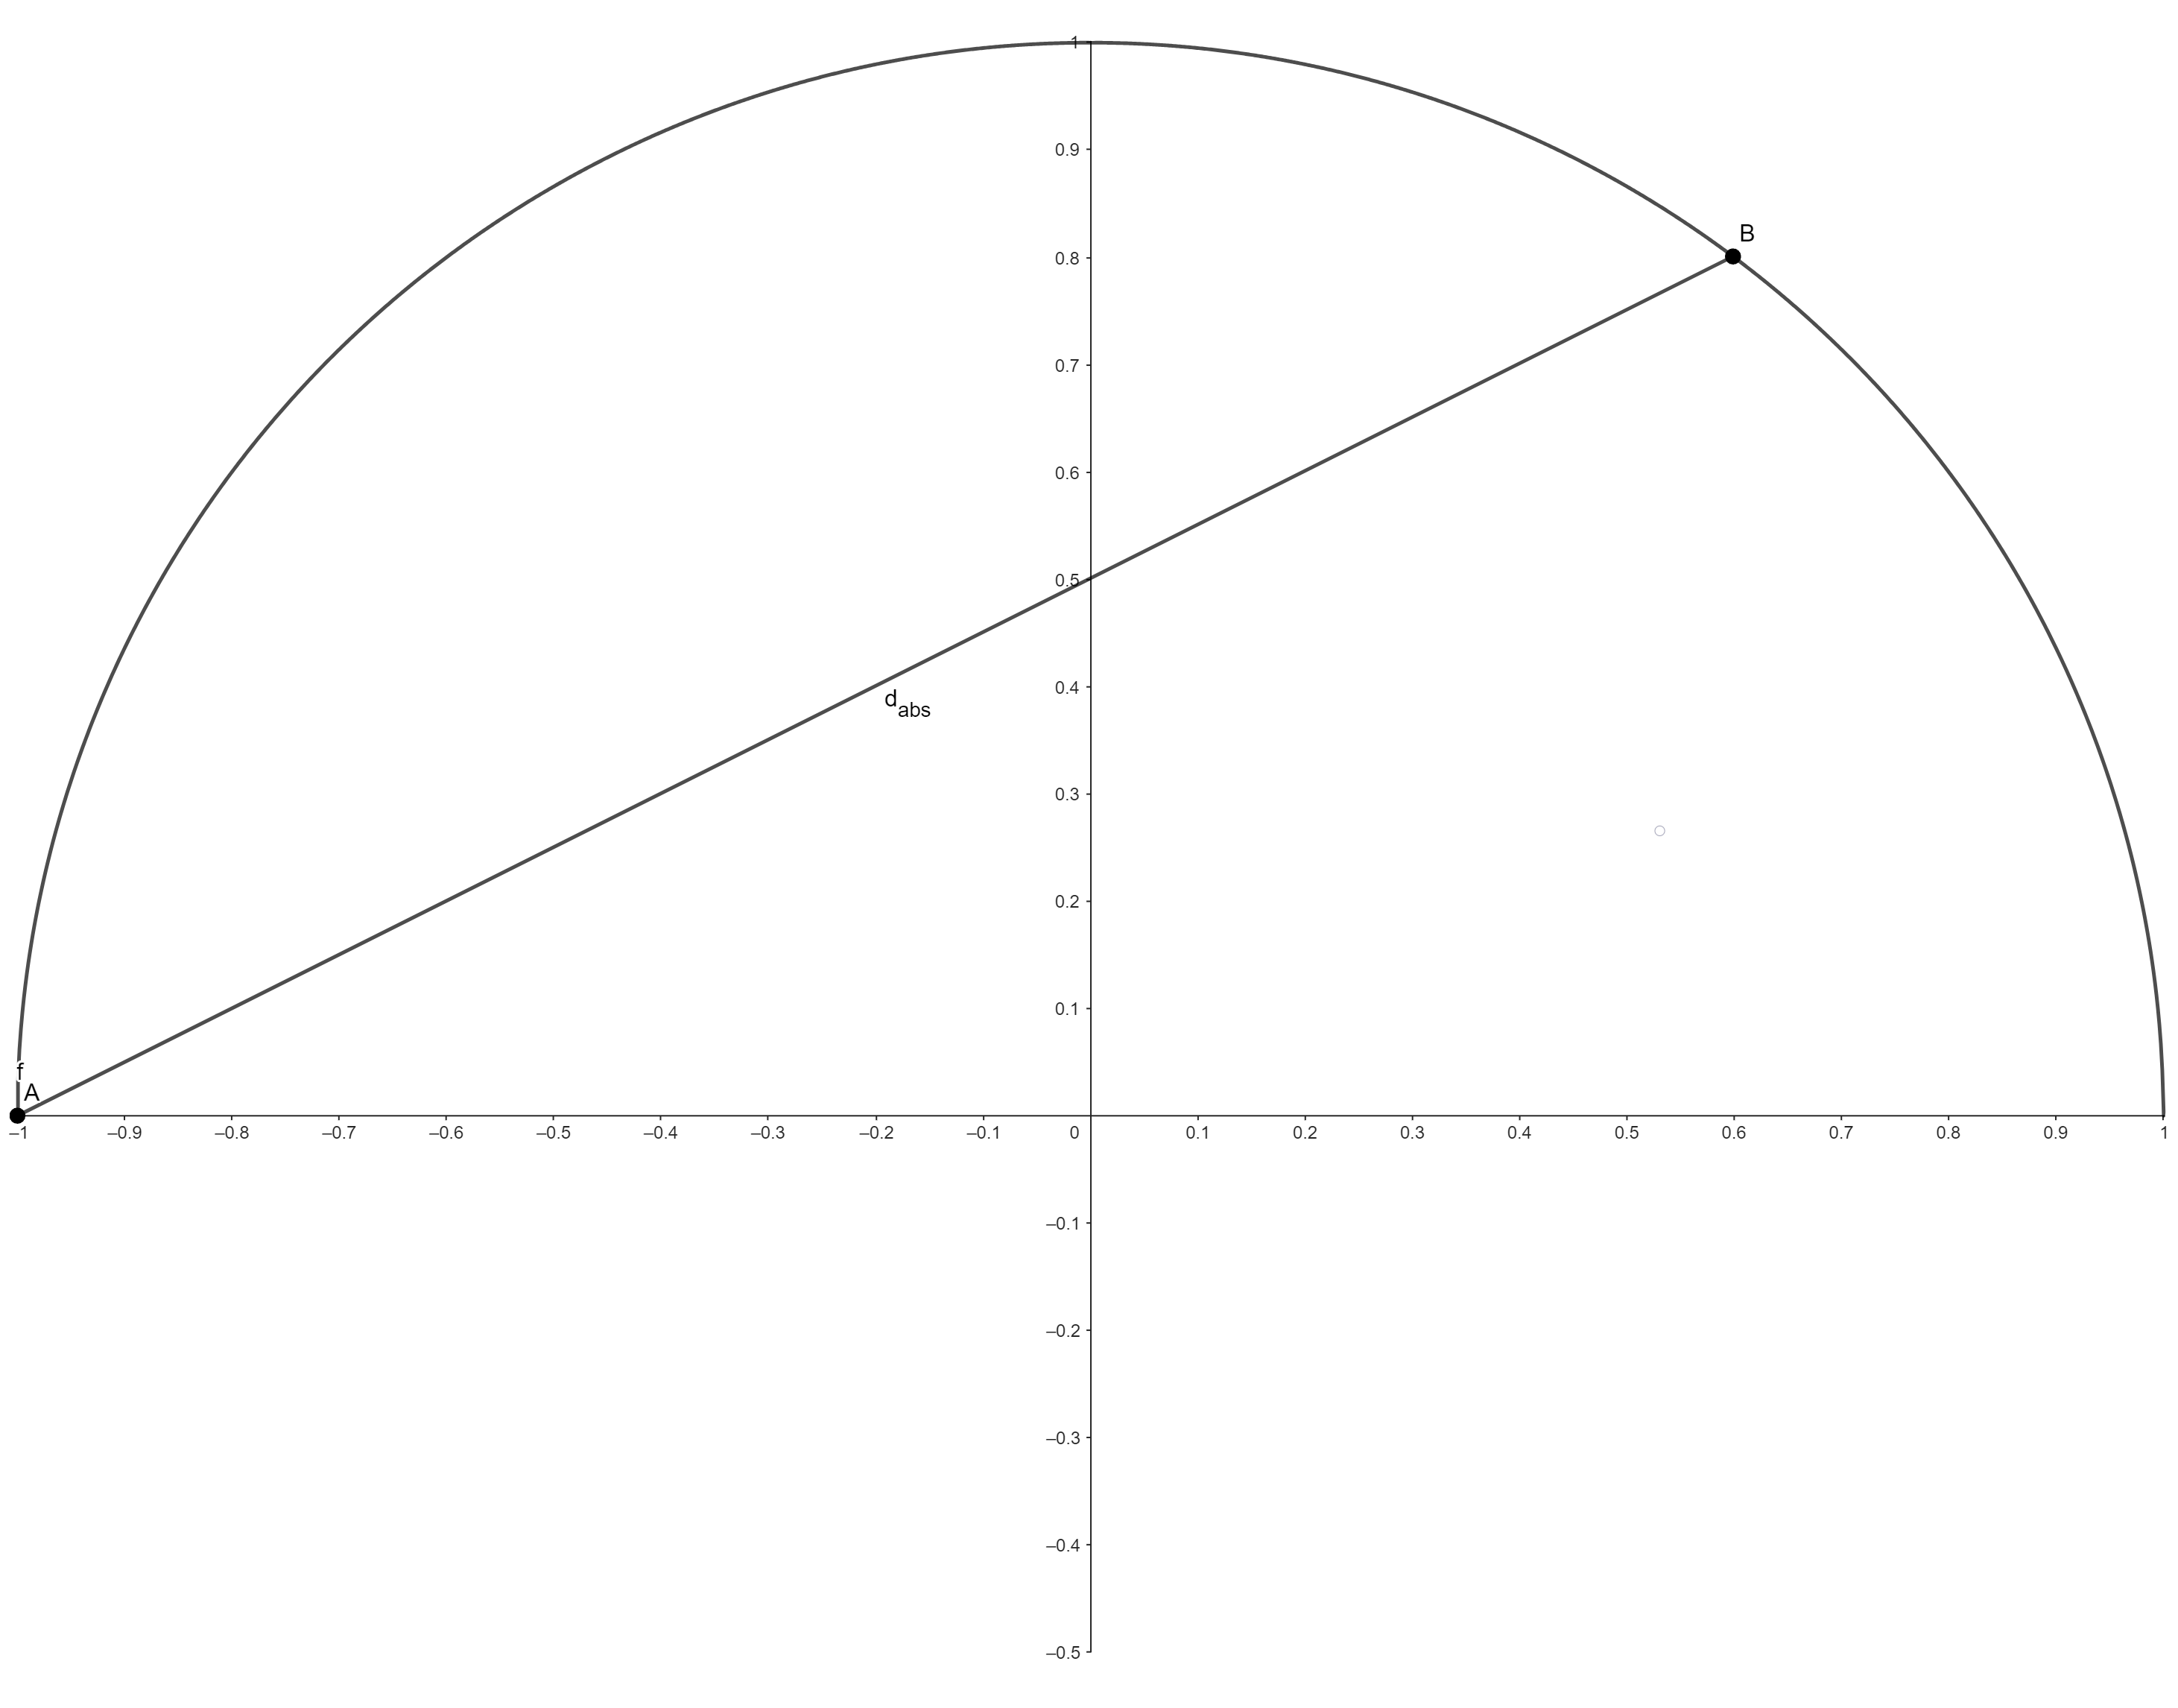
\includegraphics[scale=0.13]{angle_function.png}
    \caption{Représentation de $f$ avec $B(\approx0.6;\approx0.8)$.}
  \end{figure}

  Nous savons que: \[f^\prime(x)=\frac{-x}{\sqrt{1-x^2}}, \forall x\in]-1;1[\]

  D'après le \textbf{Théorème 3.3}, nous avons donc:

  \[d_{min}=\lambda(A,B)=\int_{-1}^{x_b} \sqrt{1+{f^\prime}^2} \,dx=\int_{-1}^{x_b} \sqrt{1+(\frac{-x}{\sqrt{1-x^2}})^2}\,dx=\int_{-1}^{x_b} \frac{1}{\sqrt{1-x^2}}\,dx\]

  On admet que:

  \[\int_{-1}^{x_b} \frac{1}{\sqrt{1-x^2}}\,dx=sin^{-1}(x)\Biggr|_{-1}^{x_b}=sin^{-1}(x_b)-sin^{-1}(-1)\]

  Soit donc $d_{min}=sin^{-1}(x_b)+\frac{\pi}{2}$.
  
  Étant dans un repère orthonormé, nous savons aussi que, d'après le Théorème de Pythagore:
  
  \[{d_{abs}}^2=(x_b-x_a)^2+(f(x_b)-f(x_a))^2 \Leftrightarrow {d_{abs}}^2=2(1+x_b) \Leftrightarrow x_b=\frac{{d_{abs}}^2}{2}-1\]

  Soit donc:

  \[d_{min}=sin^{-1}(\frac{{d_{abs}}^2}{2}-1)+\frac{\pi}{2}\]

  Si l'on définit une fonction $f_1=d_{min}, f_1:\mathbb{R}\longrightarrow \mathbb{R}, x\longmapsto f_1(x),$ pour l'\textbf{Approche 1} et $f_2=d_{min}, f_2:\mathbb{R}\longrightarrow \mathbb{R}, x\longmapsto f_2(x),$ pour l'\textbf{Approche 2} avec $x=d_{abs}$, nous avons pour $f_1(x)=2sin^{-1}(\frac{x}{2})$ et $f_2(x)=sin^{-1}(\frac{x^2}{2}-1)+\frac{\pi}{2}$.

  En comparant les courbes de la fonction $f$ des deux approches, on remarque que: \[f_2(x)=\lvert f_1(x) \rvert\]

  Cela peut se justifier par le fait que l'\textbf{Approche 2} est basée sur une fonction $f(x)\geq0 \forall x\in[-1;1]$ car un carré est toujours positif. De plus, on préfèrera l'utilisation de la fonction $f_1$ car, comme $f_1$ et $f_2$ 
  modélisent $d_{min}$ selon $d_{abs}$, il n'est pas cohérent de considérer une longueur négative, une longueur quelconque $l\in\mathbb{R^+}$. Dans $\mathbb{R^+}$, $f_1$ et $f_2$ sont semblables. Dans tous les cas, $d_{min},d_{abs}\in\mathbb{R^+}$, donc on peut négliger cette différence.
\end{proof}

\begin{theorem}
  L'appuie idéal sur la courbe d'un cercle trigonométrique est à sa circonférence divisée par 2 (soit $\pi$).
\end{theorem}

\begin{proof}
  Voici deux approches:\\
  
  \textbf{Approche 1}: Du \textbf{Théorème 4.2} découle la propriété disant que: 

  \[d_{min}=2sin^{-1}(\frac{d_{abs}}{2}) \Leftrightarrow d_{abs}=2sin(\frac{d_{min}}{2})\]

  Soit $x=d_{min}$ et une fonction $f:\mathbb{R}\longrightarrow \mathbb{R}, x\longmapsto f(x)$ tel que  $f(x)=d_{abs}$. Nous avons donc:

  \[f(x)=2sin(\frac{x}{2})\]

  Ainsi que:

  \[f^\prime(x)=cos(\frac{x}{2})\]

  On admet que $f^\prime(x)=0$ lorsque $x=\pi$ dans l'intervalle $I=[0;2\pi]$, soit donc un maximum avec $f(\pi)=2 \Leftrightarrow d_{abs}=2$ pour $d_{min}=\pi$. 

  En d'autres termes, toutes les valeurs $d_{min}$ n'amèneront pas aussi loin que son diamètre, comme $d_{abs}=2$. Cela laisse donc considérer l'idée d'appuyer sur le bouton à ce maximum afin d'effectuer un nouveau cercle trigonométrique. 
  (cela laisse aussi supposer, que par récurrence, il faudra toujours appuyer sur le bouton à la moitié de la circonférence pour progresser efficacement dans le plan).\\

  \textbf{Approche 2}: En se basant plus sur la logique, on remarque bien qu'afin d'amener notre électron le plus loin possible, il faut arrêter le trajet et appuyer sur le bouton
  au demi-cercle. En effet, si l'on appuie au délà de la circonférence, nous effectuons un trajet plus long avec une distance absolue $d_{abs}$ plus courte. Voici une illustration:

  \begin{figure}[H]
    \centering
    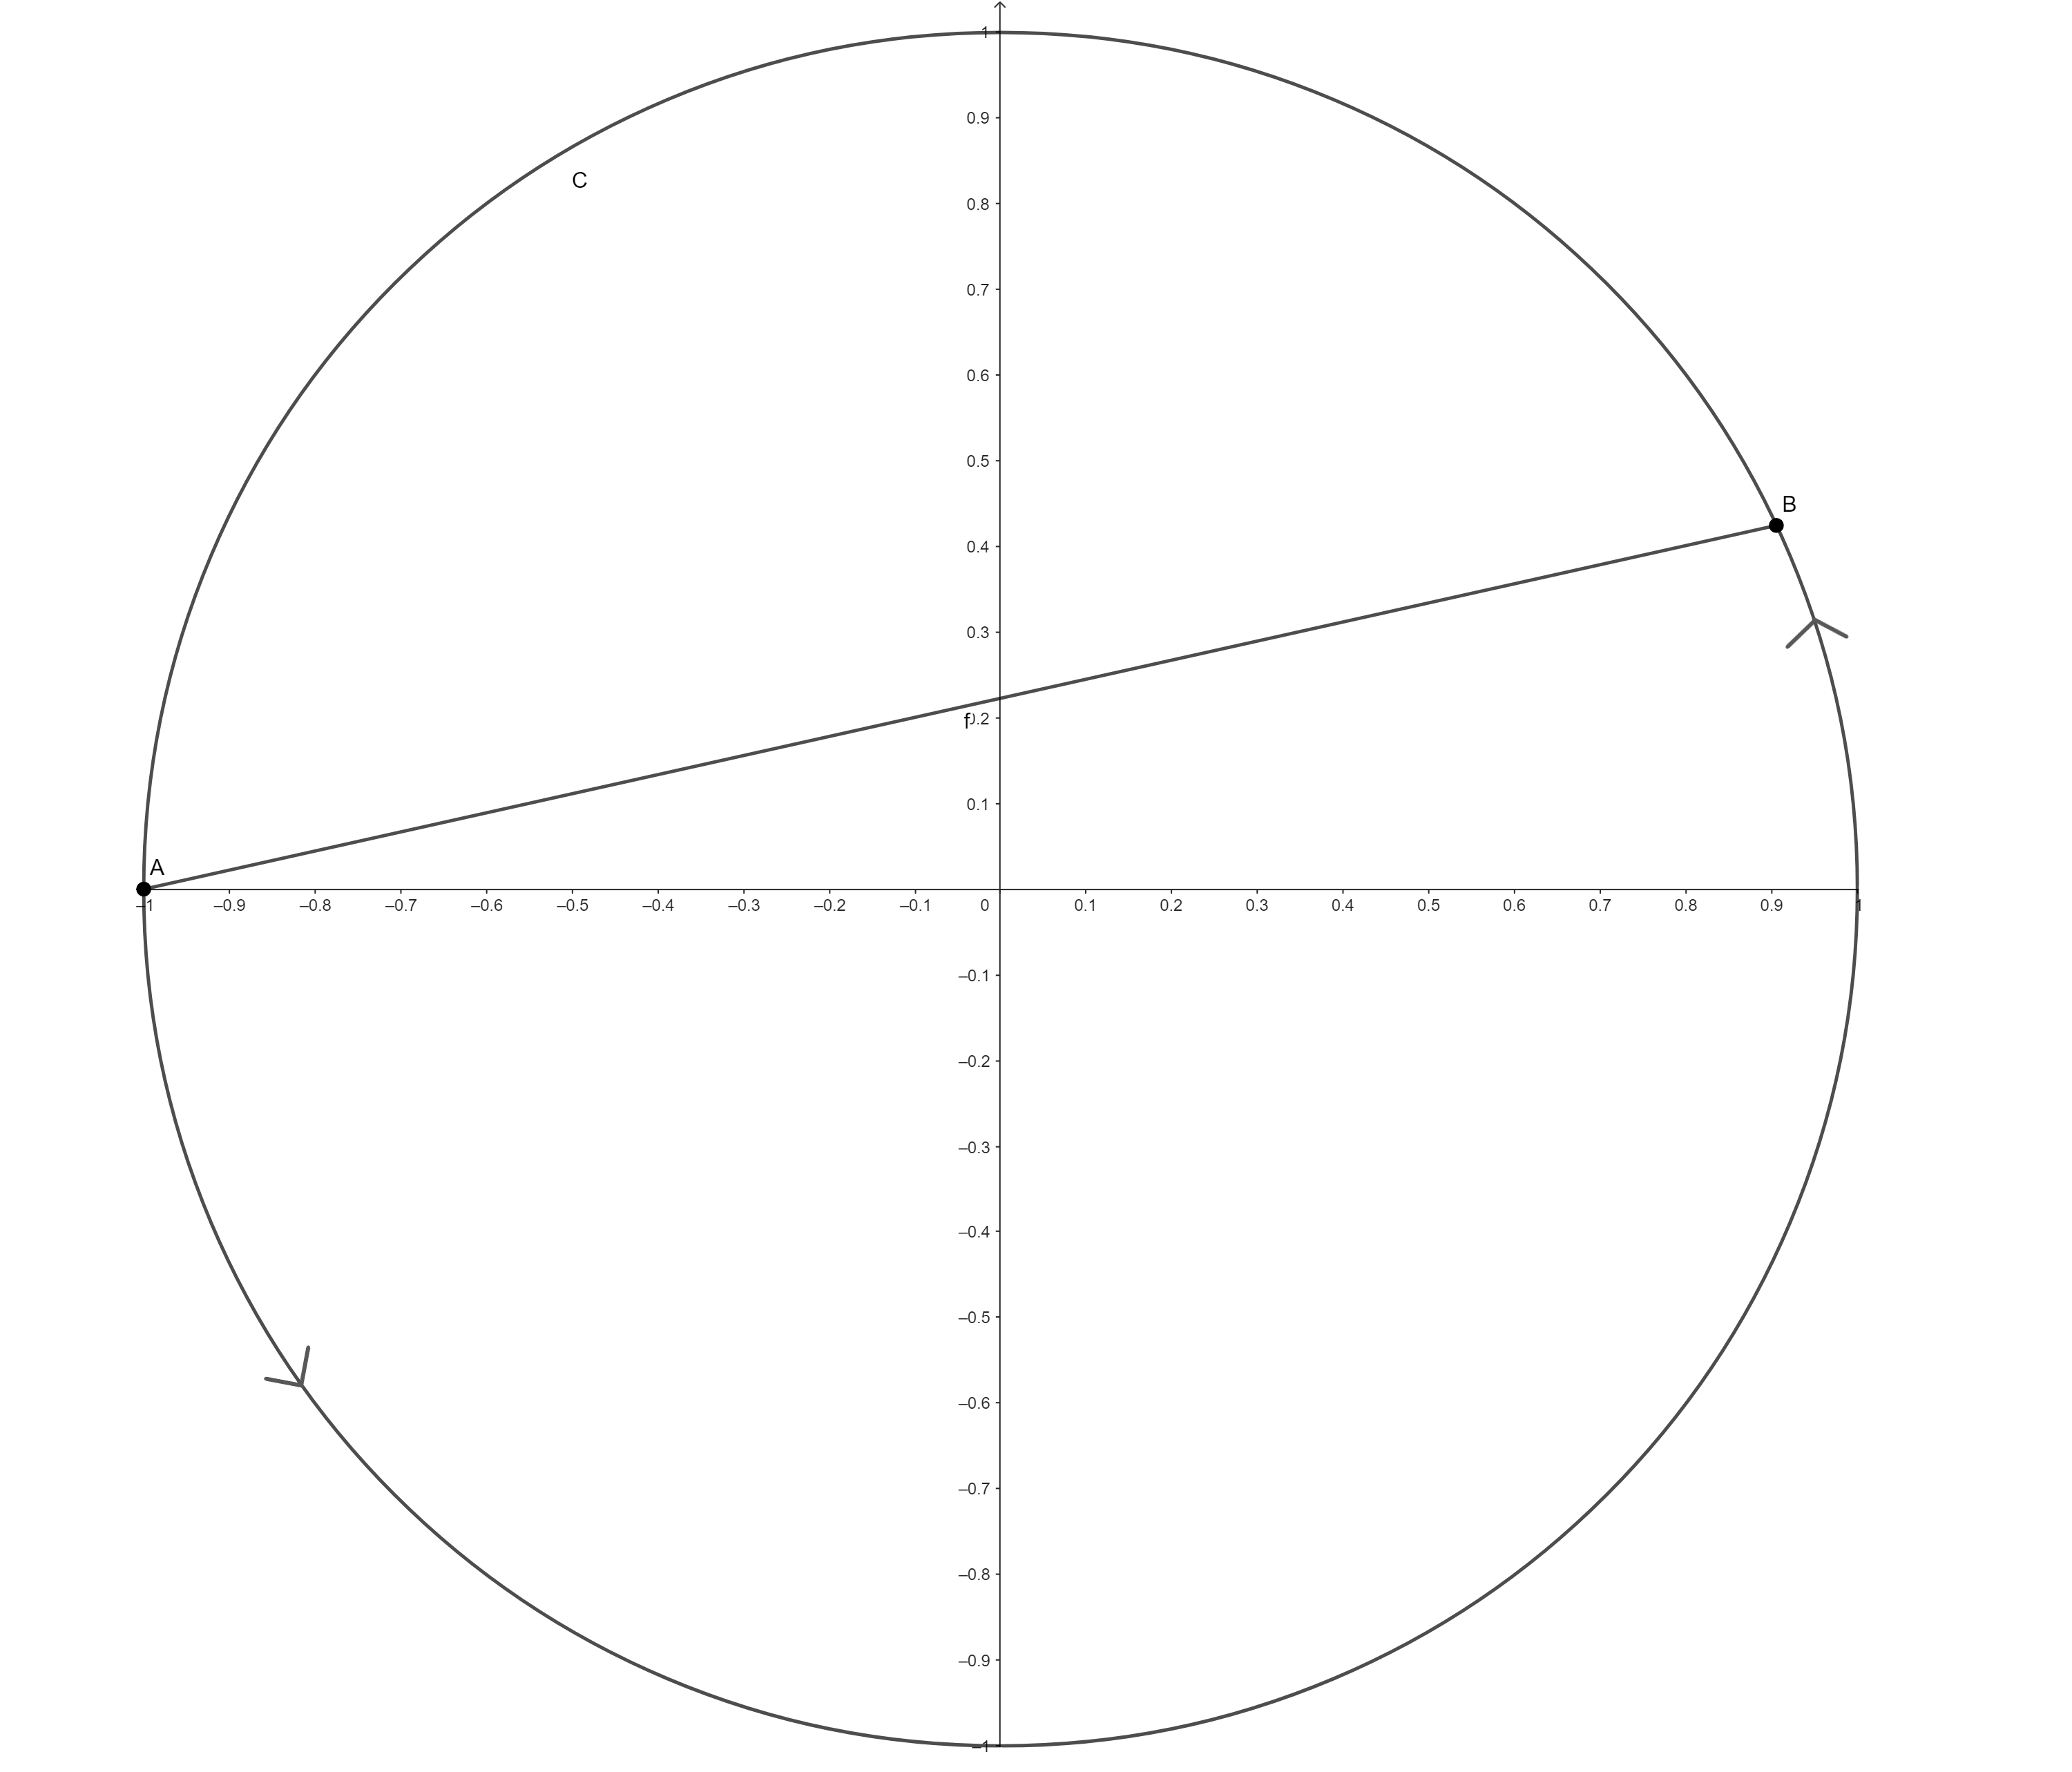
\includegraphics[scale=0.13]{ab_circle1.png}
    \caption{Un trajet long avec $d_{abs}=1.95$.}
  \end{figure}

  \begin{figure}[H]
    \centering
    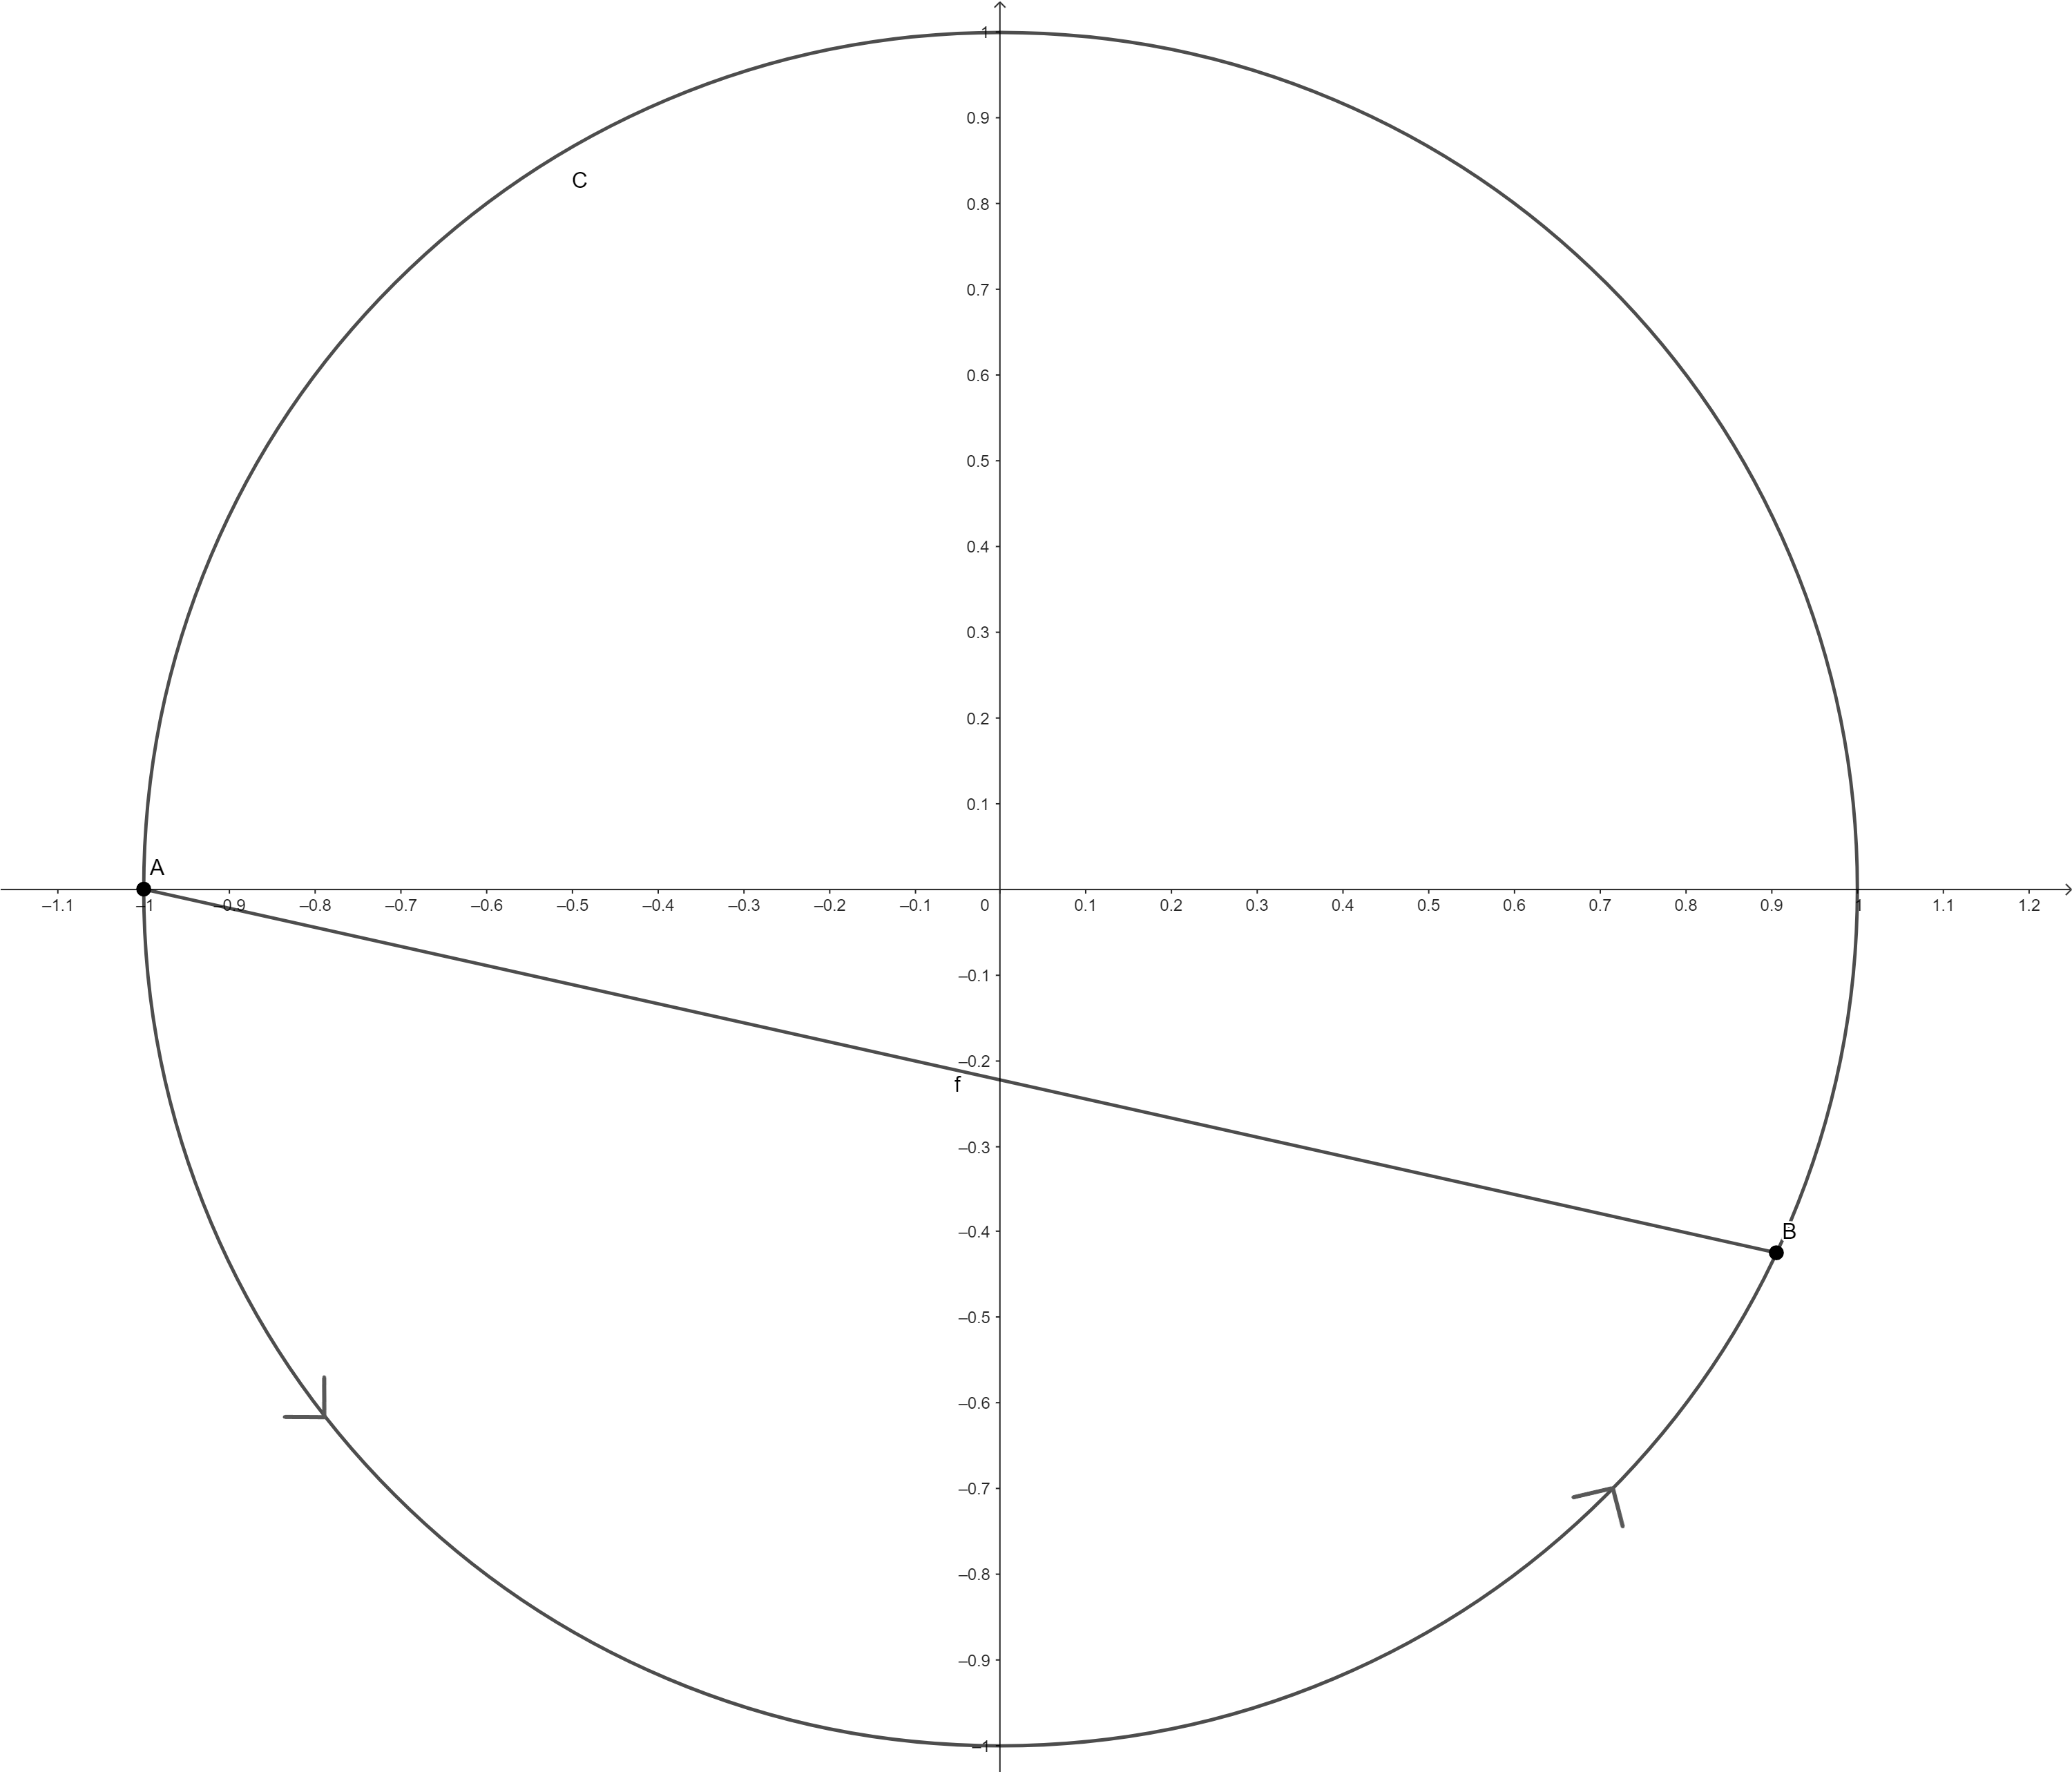
\includegraphics[scale=0.13]{ab_circle2.png}
    \caption{Un trajet moins long avec $d_{abs}=1.95$.}
  \end{figure}

  On comprend donc qu'avec la possibilité de choisir l'orientation initiale, on peut toujours s'arranger pour former un demi-cercle trigonométrique amenant l'électron de $A$ vers $B$. En considérant ce demi-cercle, on remarque bien que le trajet 
  amenant le plus loin est à la moitié de sa circonférence, soit $\pi$, et qu'il n'est pas nécessaire de laisser l'électron progresser au delà. On considère donc l'appuie du bouton à un tel emplacement.

  \begin{figure}[H]
    \centering
    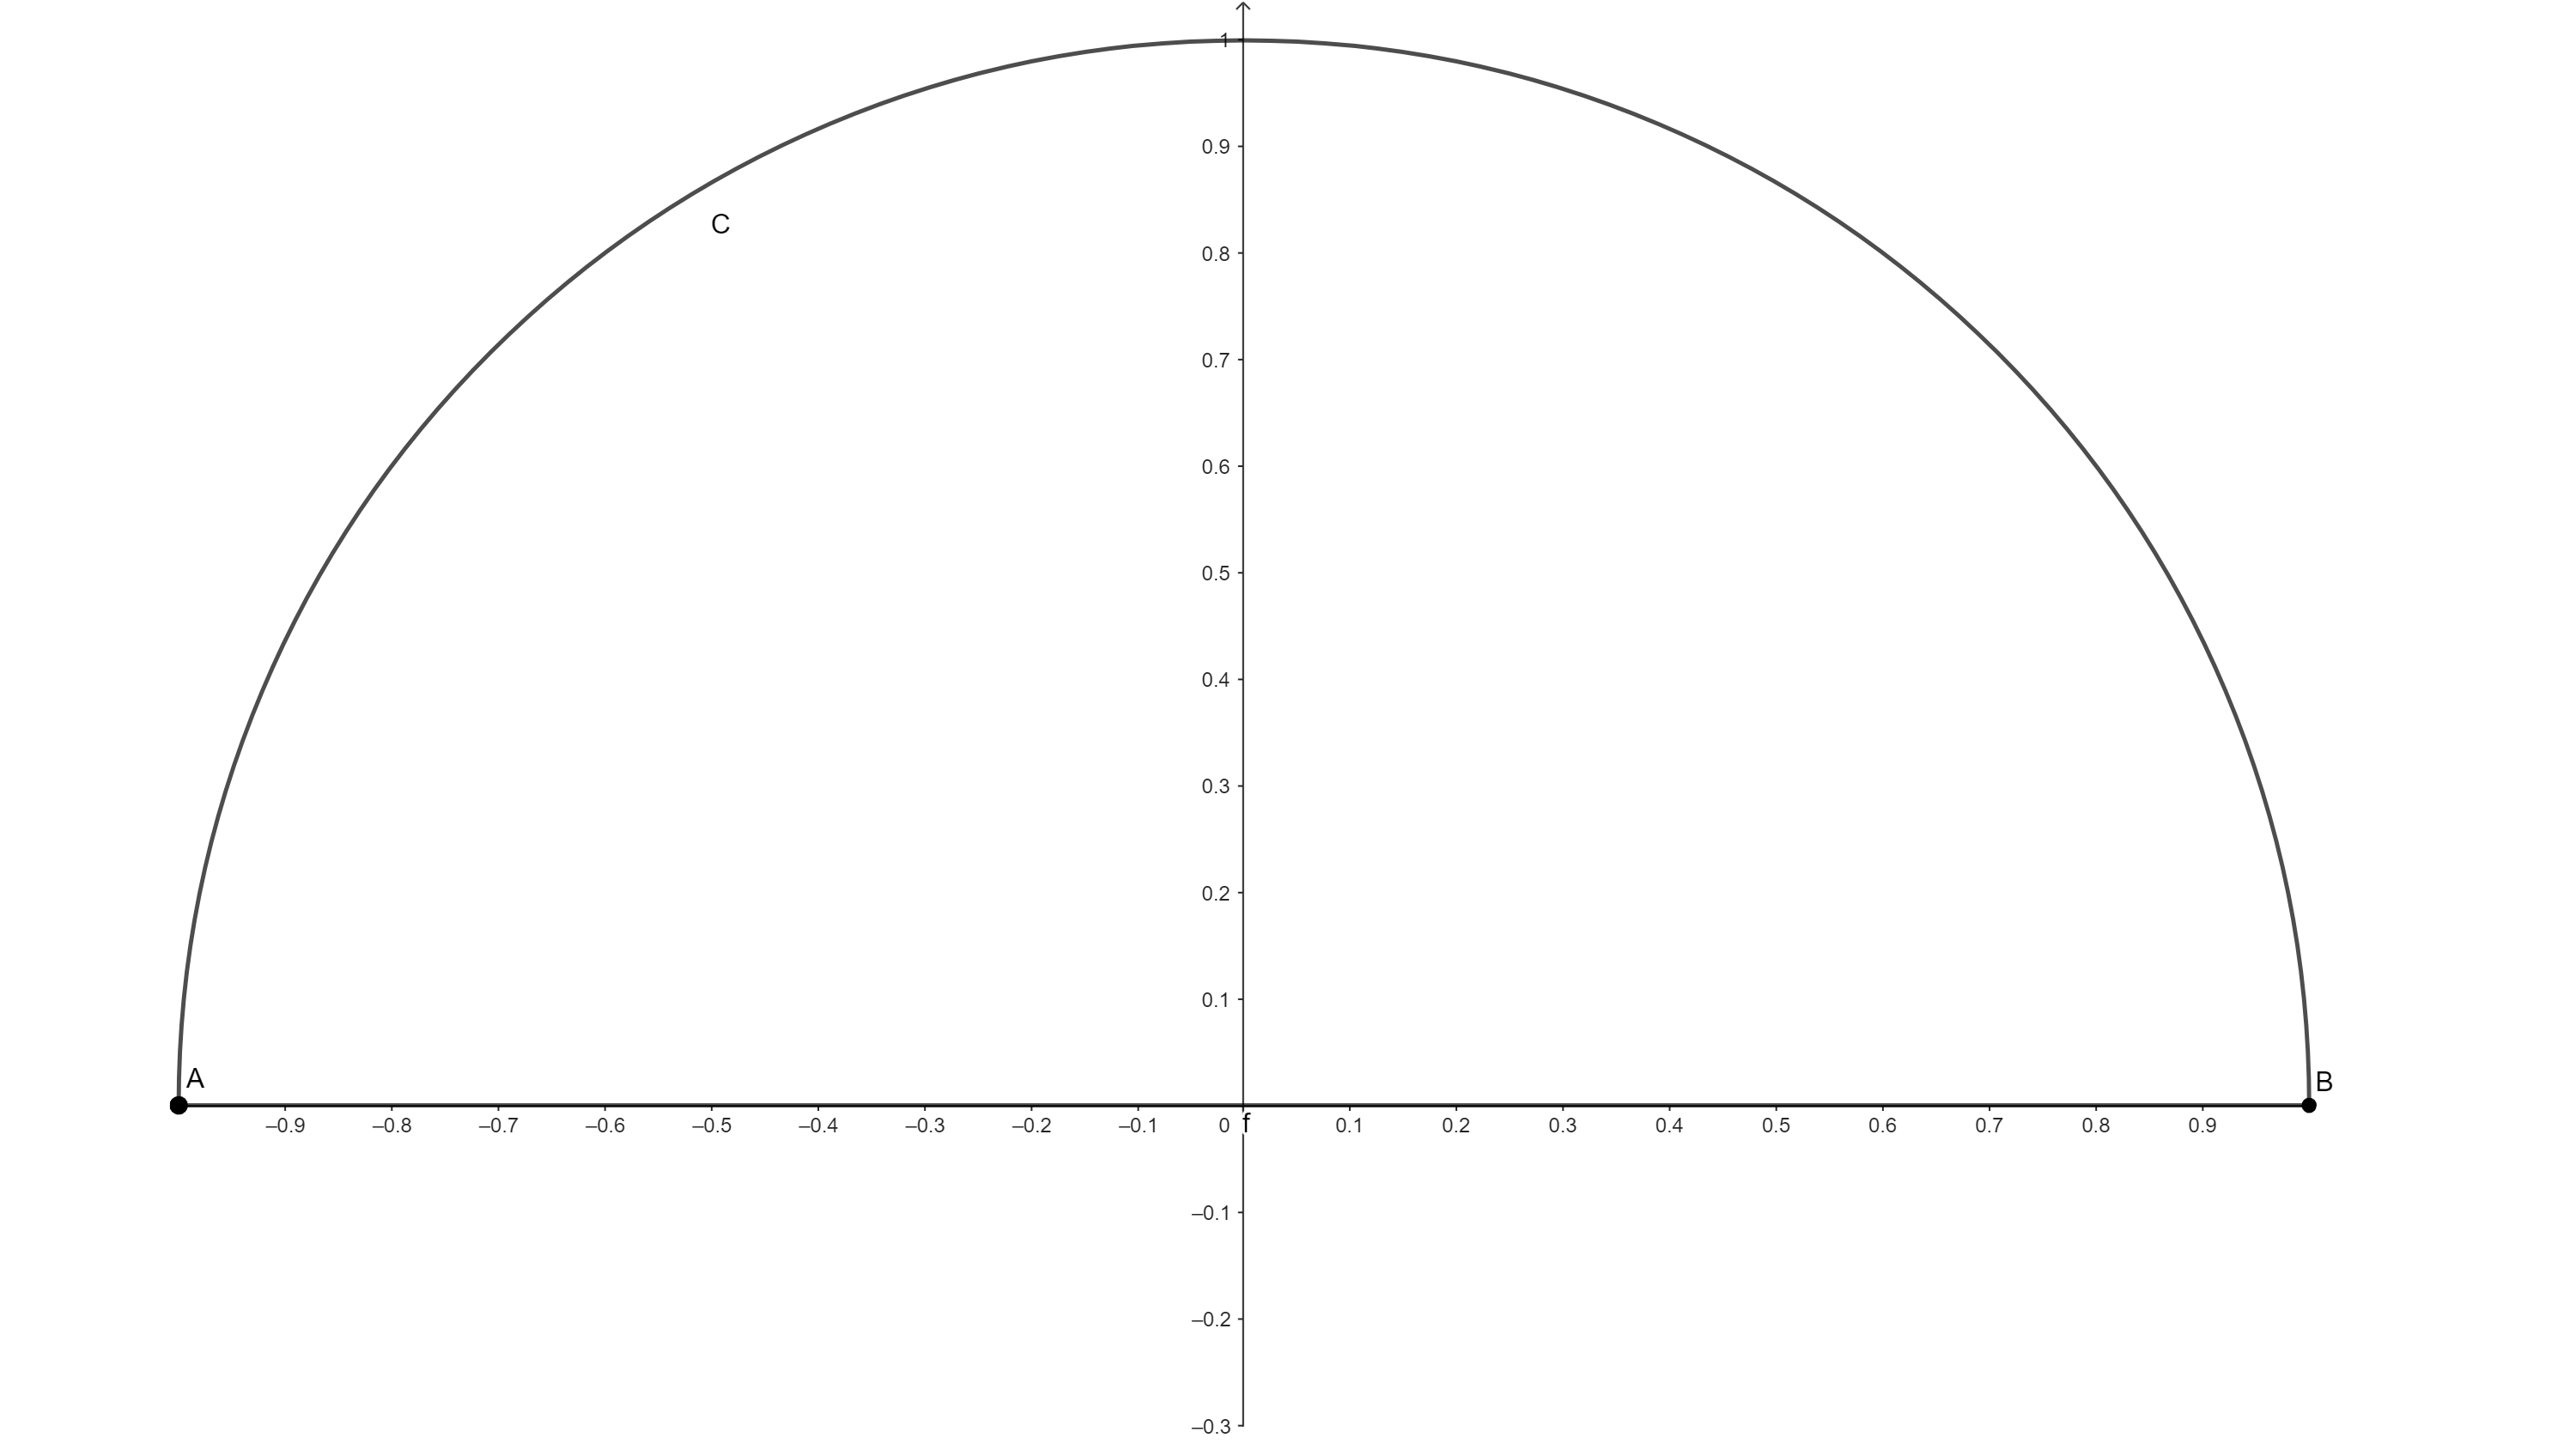
\includegraphics[scale=0.13]{ab_circle.png}
    \caption{Un trajet idéal avec $d_{abs}=2$, le diamètre étant le maximum.}
  \end{figure}

\end{proof}

\begin{theorem}
  Soit A,B deux points dans un plan orthonormé. Avec un trajet formant un demi-cercle trigonométrique perpétuel de $A$ à $B$ et la possibilité de changer de direction à des points $C_0, C_1$, ... $C_{n-1}, C_{n}$ (selon l'énoncé),$n\in\mathbb{N}$, le trajet le plus court
  est le demi-cercle trigonométrique perpétuel de $A$ à $B$, avec $A,C_0, C_1$, ... $C_{n-1}, C_{n}$ et $B$ alignés.
\end{theorem}

\begin{proof}
  On comprend qu'avec le \textbf{Théorème 3.3}, afin de maximiser la distance minimale entre $A$ et $B$, il faut que la courbe passant par $A$ et $B$ aie une forme se rapprochant d'un droite. 
  Le problème réside donc dans la question: Il y a t'il un moyen de conformer les points $A$, $C_0, C_1, ... C_n$ et $B$ afin de faire une courbe se rapprochant d'une droite, où en d'autres termes, est-il possible que $d_{min}\approx d_{abs}$.\\

  Connaissant, d'après le \textbf{Théorème 4.3}, qu'il faut appuyer idéalement à la moitié de la circonférence, on peut dors-et-déjà déduire le fait que par récurrence, appuyer perpétuellement à la moitié de la circonférence amènera l'électron le plus loin 
  possible (soit donc former des demi-cercles trigonométrique perpétuels). Mais, nous pouvons affirmer ce principe par d'autres justifications:\\

  \textbf{Justification 1}: En prenant une version simplifiée du problème. On définit un repère orthonormé $(A;I;J)$ tel que \overrightarrow{AJ} $\perp$ \overrightarrow{AB}. On considère donc les points $A(x_a=0,y_a=0)$ et $B(x_b,y_b=0)$.
  Prenons le cas où $n_{bouton}=2$ et les points $C$ et $D$, l'emplacement de l'électron lorsque le bouton a été appuyé.

  \begin{figure}[H]
    \centering
    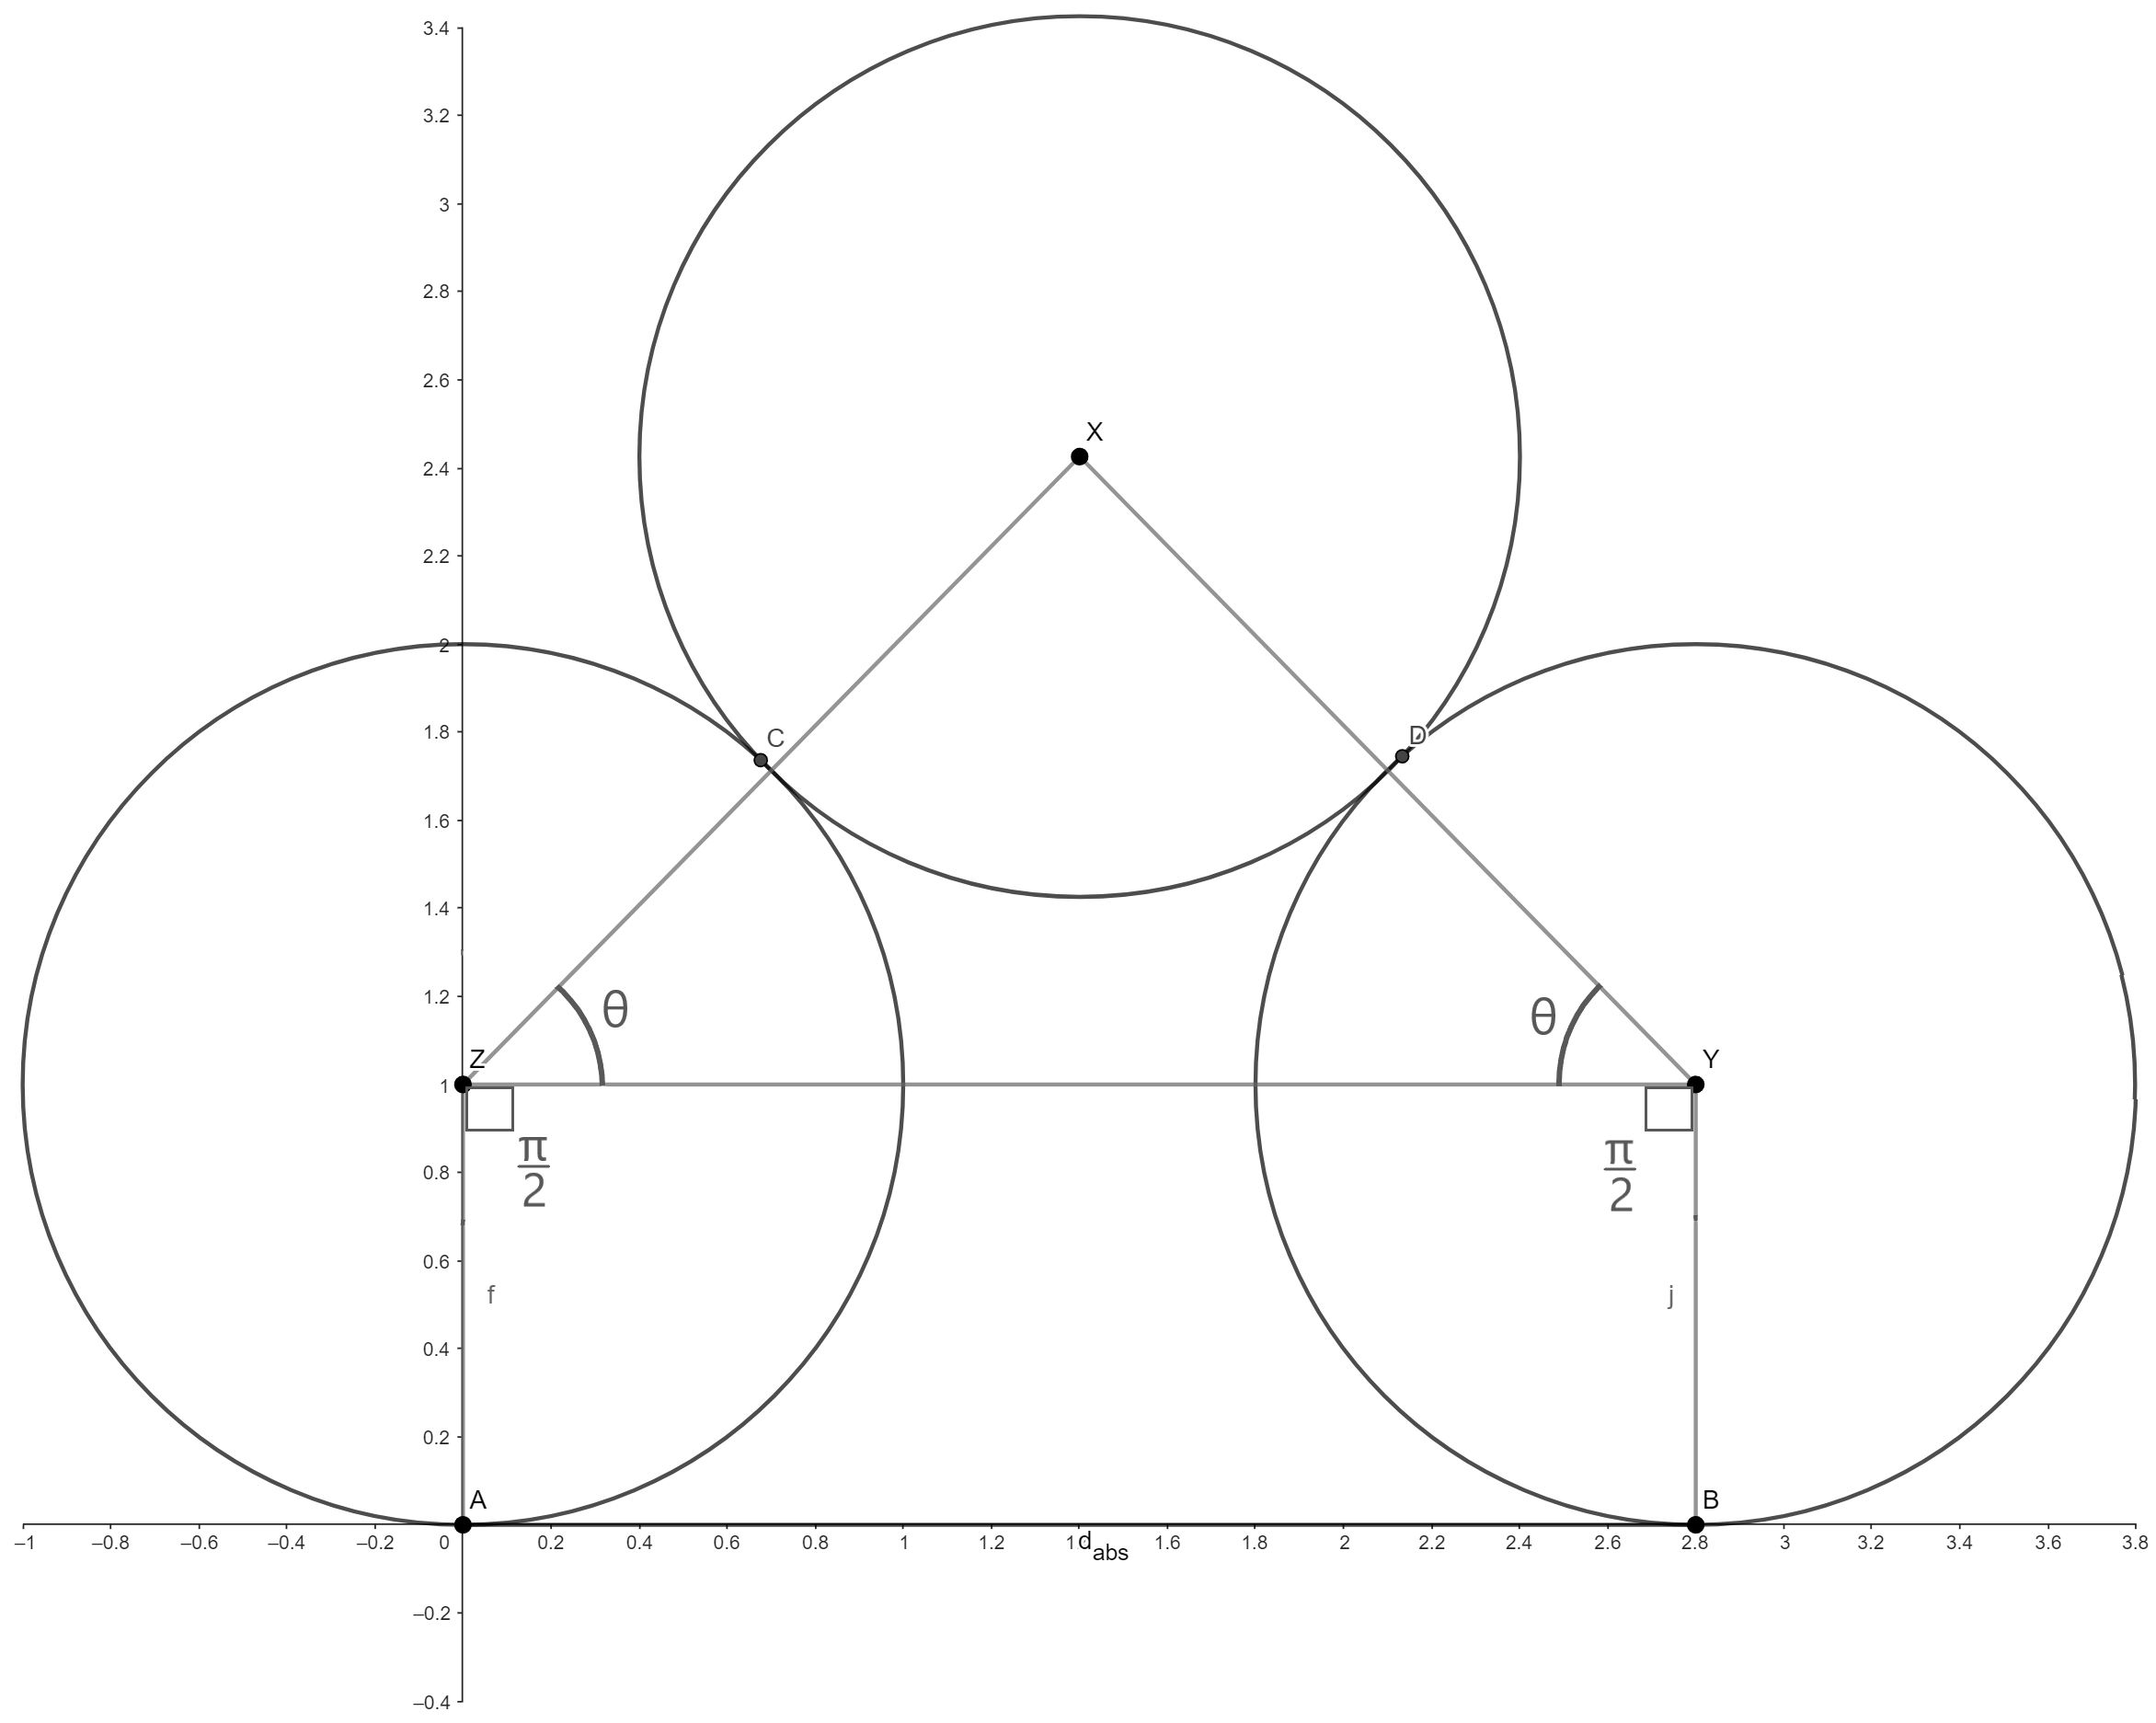
\includegraphics[scale=0.2]{three_circles.png}
    \caption{}
  \end{figure}

  \textbf{Justification 2}:

  \textbf{Généralisation des justifications}:
  
\end{proof}

\section{Réponse à la Question 1}

\begin{theorem}
  Soit $A,B$ deux points dans un plan quelconque. Il est toujours possible d'atteindre $B$ en partant de $A$ en formant des demi-cercles trigonométrique perpétuels et en pouvant choisir l'orientation initiale.
\end{theorem}

\begin{proof}
  On considère un point $A$ dans un plan quelconque et $C_a$, le cercle trigonométrique passant par $A$.

  À $n_{bouton}=0$, pouvant choisir l'orientation de base du cercle trigonométrique, on en déduit que l'on peut former un nouveau cercle $C_{a^\prime}$ selon les possibilités d'orientation.  $C_{a^\prime}$ a donc pour rayon $r_{a^\prime}\in\mathbb{R^+}, r_{a^\prime}=2$, étant le 
  diamètre du cercle trigonométrique. Cela couvre donc tous les points ayant une distance $d=2$ de $A$, soit donc une surface de $4\pi$.

  Après avoir parcouru un trajet $T=\pi$. D'après le \textbf{Théorème 4.3}, on considère le fait d'appuyer sur le bouton ($n_{bouton}=1$) pour pouvoir progresser dans le plan. Par le même raisonnement que lorsque $n_{bouton}=0$,
  on en déduit que l'on peut former un nouveau cercle $C_{a^{\prime\prime}}$ selon les possibilités d'orientation.  $C_{a^{\prime\prime}}$ a donc pour rayon $r_{a^{\prime\prime}},=2r_{a^\prime}=4$ et une surface de $16\pi$.

  Par récurrence, on déduit que l'on peut toujours former un cercle $C_k$ de rayon $r_k=2(n_{bouton}+1) \implies$ lorsque $n_{bouton}\to+\infty$, $r_k\to+\infty \implies {\pi}r_k^2\to+\infty$, couvrant ainsi l'ensemble du plan.

  On comprend donc qu'il est possible à partir du point $A$ d'atteindre n'importe quel point $B$ dans le plan.


  Voici une représentation visuelle permettant d'expliquer le raisonnement:
  \begin{figure}[H]
    \centering
    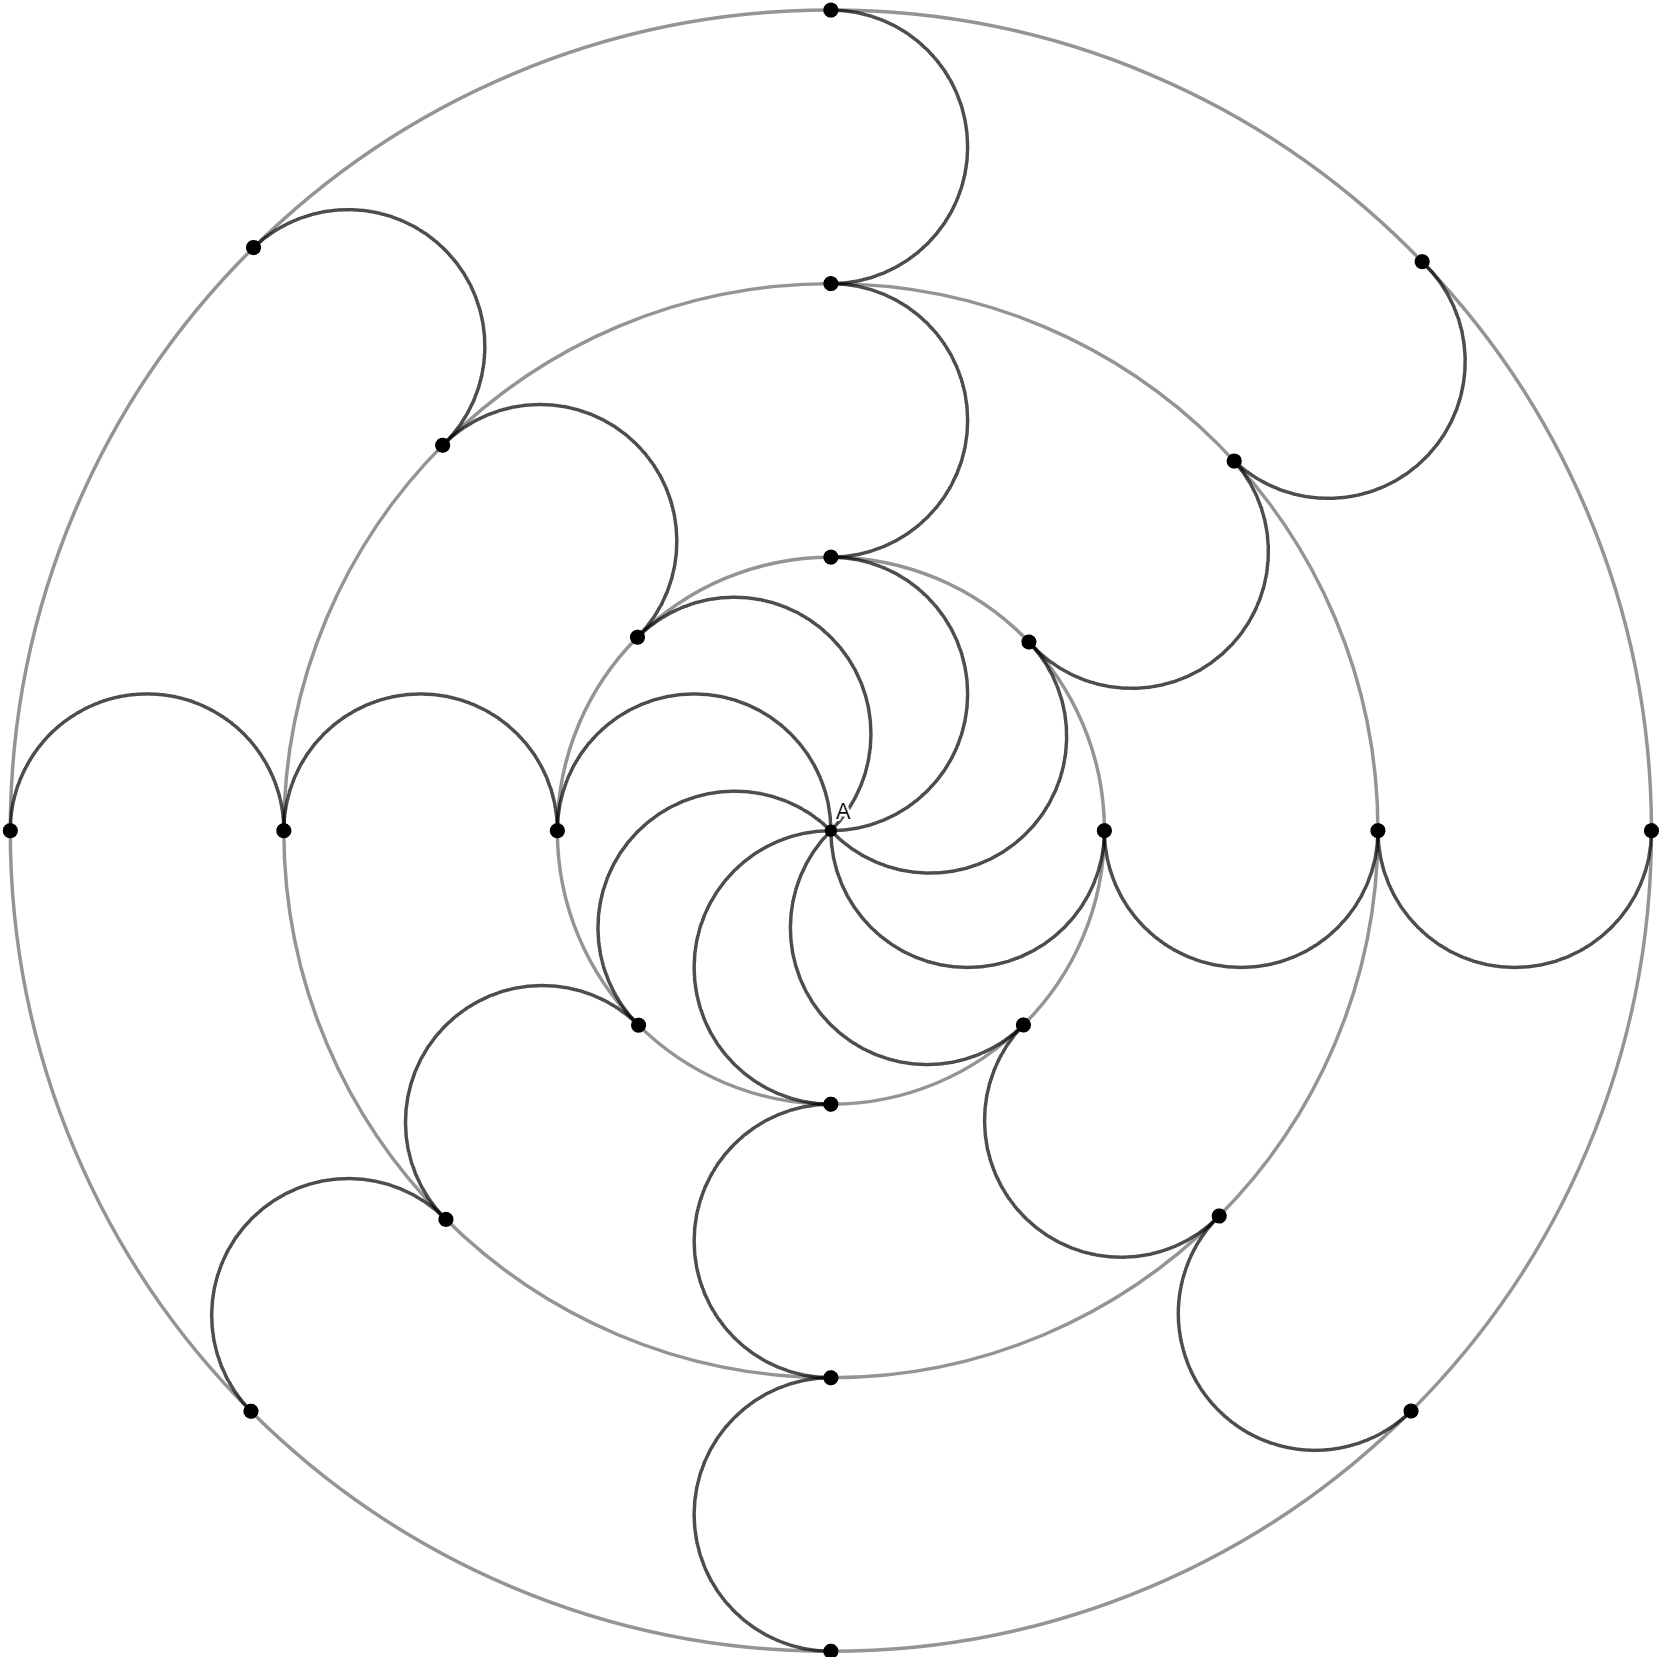
\includegraphics[scale=0.27]{visualization.png}
    \caption{Représentations des moyens d'atteindre $B$ en partant de $A$ avec une division=8 selon l'orientation (les points des courbes circulaires ont donc un angle de 45° entre eux selon le point $A$) avec $n_{bouton}=2$. 
    Les points noirs sont des points $B$ avec la longueur du segment [AB] un multiple de $2$.}
  \end{figure}
\end{proof}
\end{document}